% VUT FIT MITAI
% MSZ 2021/2022
% Author: Vladimir Dusek
% Login: xdusek27

%%%%%%%%%%%%%%%%%%%%%%%%%%%%%%%%%%%%%%%%%%%%%%%%%%%%%%%%%%%%%%%%%%%%%%%%%%%%%%%%

% Path to figures
\graphicspath{{bms/bezdratove_lokalni_site/figures}}

%%%%%%%%%%%%%%%%%%%%%%%%%%%%%%%%%%%%%%%%%%%%%%%%%%%%%%%%%%%%%%%%%%%%%%%%%%%%%%%%

\chapter{BMS -- Bezdrátové lokální sítě (Wifi, Bluetooth).}

% Otazka MSZ 2020, 113 MSK
% [Ocenasek] Bezpecnost bezdratovych siti, chvili me nechal mluvit, tak jsem rekl neco k WEPu, pak uz to bylo stylem otazka odpoved. Zajimala ho proudova sifra WEPu, TKIP ve WPA, WPA enterprise a 802.1x, ale vetsinou chtel vedet spis veci obecneho charakteru, napr. jake jsou vyhody WPA enterprise oproti PSK a tak

%%%%%%%%%%%%%%%%%%%%%%%%%%%%%%%%%%%%%%%%%%%%%%%%%%%%%%%%%%%%%%%%%%%%%%%%%%%%%%%%

\section{Zdroje}

\begin{compactitem}
    \item \path{08-bezdratove_lan.pdf}
    \item \path{BMS_2020-12-02.mp4} % Todo: cas 7:35
    \item \path{BMS_2020-12-09.mp4}
\end{compactitem}

%%%%%%%%%%%%%%%%%%%%%%%%%%%%%%%%%%%%%%%%%%%%%%%%%%%%%%%%%%%%%%%%%%%%%%%%%%%%%%%%

\section{Bezdrátová komunikace}

\begin{compactitem}
    \item Radiové vlny je elektromagnetické vlnění ve frekvenčním rozsahu 300\,GHz -- 30\,Hz.
    \item Bitová rychlost -- Počet přenesených bitů za časovou jednotku.
    \item Baudová rychlost -- Počet přenesených signálových jednotek za časovou jednotku (baud rate $\leq$ bit rate).
    \item Princip bezdrátové komunikace a jednotlivé fáze přenosu:
\end{compactitem}

\begin{compactenum}
    \item \textbf{Kódování hlasu a digitalizace} \begin{compactitem}
        \item Z analogového hlasu uděláme digitální signál.
        \item Velká redundance, provádíme kompresy.
        \item Dojde ke ztrátě nějakých informací a přidání šumu (kvantizační šum) při dekódování.
        \item Např. pulzně kódová modulace (PCM, \textit{pulse-code modulation}).
    \end{compactitem}

    \item \textbf{Kódování kanálu} \begin{compactitem}
        \item Data jsou přenášena přes rádiové kanály, které jsou nespolehlivé (data se mohou ztratit, bit může \uv{přeskočit}, \dots).
        \item Počítáme s tím, zavádíme redundanci tak, aby bylo možné většinu chyb opravit. \begin{compactitem}
            \item Chceme minimalizovat opětovné přenášení (to je problém).
            \item Detekce chyb pomocí BER -- Bit Error Rate, FER -- Frame Error Rate.
        \end{compactitem}
        \item Zvyšuje se tím výrazně objem dat.
        \item Metody: \begin{compactitem}
            \item Blokové korekční kódy (Hammingův kód) -- vstup je rámec, výstup je původní rámec + zabezpečovací bity.
            \item Konvoluční korekční kódy -- nezná pojem rámec, vstupují bity a vystupují bity rychleji.
            \item Turbo korekční kódy.
        \end{compactitem}
    \end{compactitem}

    \item \textbf{Prokládání (\textit{interleaving})} \begin{compactitem}
        \item Pokud se na kanálu objevuje nějaké rušení, tak je většinou impulsní a zaruší se několik bitů vedle sebe.
        \item To se nelíbí mechanismům kódování kanálu, ty mají rády pokud je zarušen \uv{sem tam} nějaký bit, ale ne shluk vedle sebe.
        \item Zabraňujeme tomu tak, že prohazujeme pořadí jednotlivých bitů.
    \end{compactitem}

    \item \textbf{Šifrování dat} \begin{compactitem}
        \item Může být v různé fázi, není shoda.
        \item Umístění šifrování tak jak ve schématu je problém, jelikož se mohou objevit chyby díky přenosu, což se většine šifrovacích algoritmů nelíbí, proto by dávalo smysl to umístit až za (de)kódování kanálu.
    \end{compactitem}

    \item \textbf{Modulace} \begin{compactitem}
        \item Dostat náš signál do analogové podoby pro přenos a na potřebnou frekvenci (úprava frekvencí, amplitud, fází).
        \item Také prováděn multiplexing (přenášení více signálů přes jednu anténu).
    \end{compactitem}

    \item \textbf{Přenos signálu přes telekomunikační síť} \begin{compactitem}
        \item Jak bylo řečeno výše, jde o nespolehlivý přenos přes rádiové (nebo historicky infračervené) záření.
    \end{compactitem}

    \item \textbf{Demodulace} \begin{compactitem}
        \item Dostat signál z podoby vhodné pro přenos na podobu vhodnou pro dekódování (úprava frekvencí, amplitud, fází).
        \item Prováděn demultiplexing.
    \end{compactitem}

    \item \textbf{Dešifrování} \begin{compactitem}
        \item Dešifrování, platí to stejné jako u šifrování.
    \end{compactitem}

    \item \textbf{Prokládání (\textit{deinterleaving})} \begin{compactitem}
        \item Překládání bitů analogicky k prokládání na druhé straně.
    \end{compactitem}

    \item \textbf{Dekódování kanálu} \begin{compactitem}
        \item Opravení chyb.
    \end{compactitem}

    \item \textbf{Dekódování hlasu} \begin{compactitem}
        \item Pokud chceme řeč, tak převod do analogové podoby.
    \end{compactitem}
\end{compactenum}

\begin{figure}[H]
    \centering
    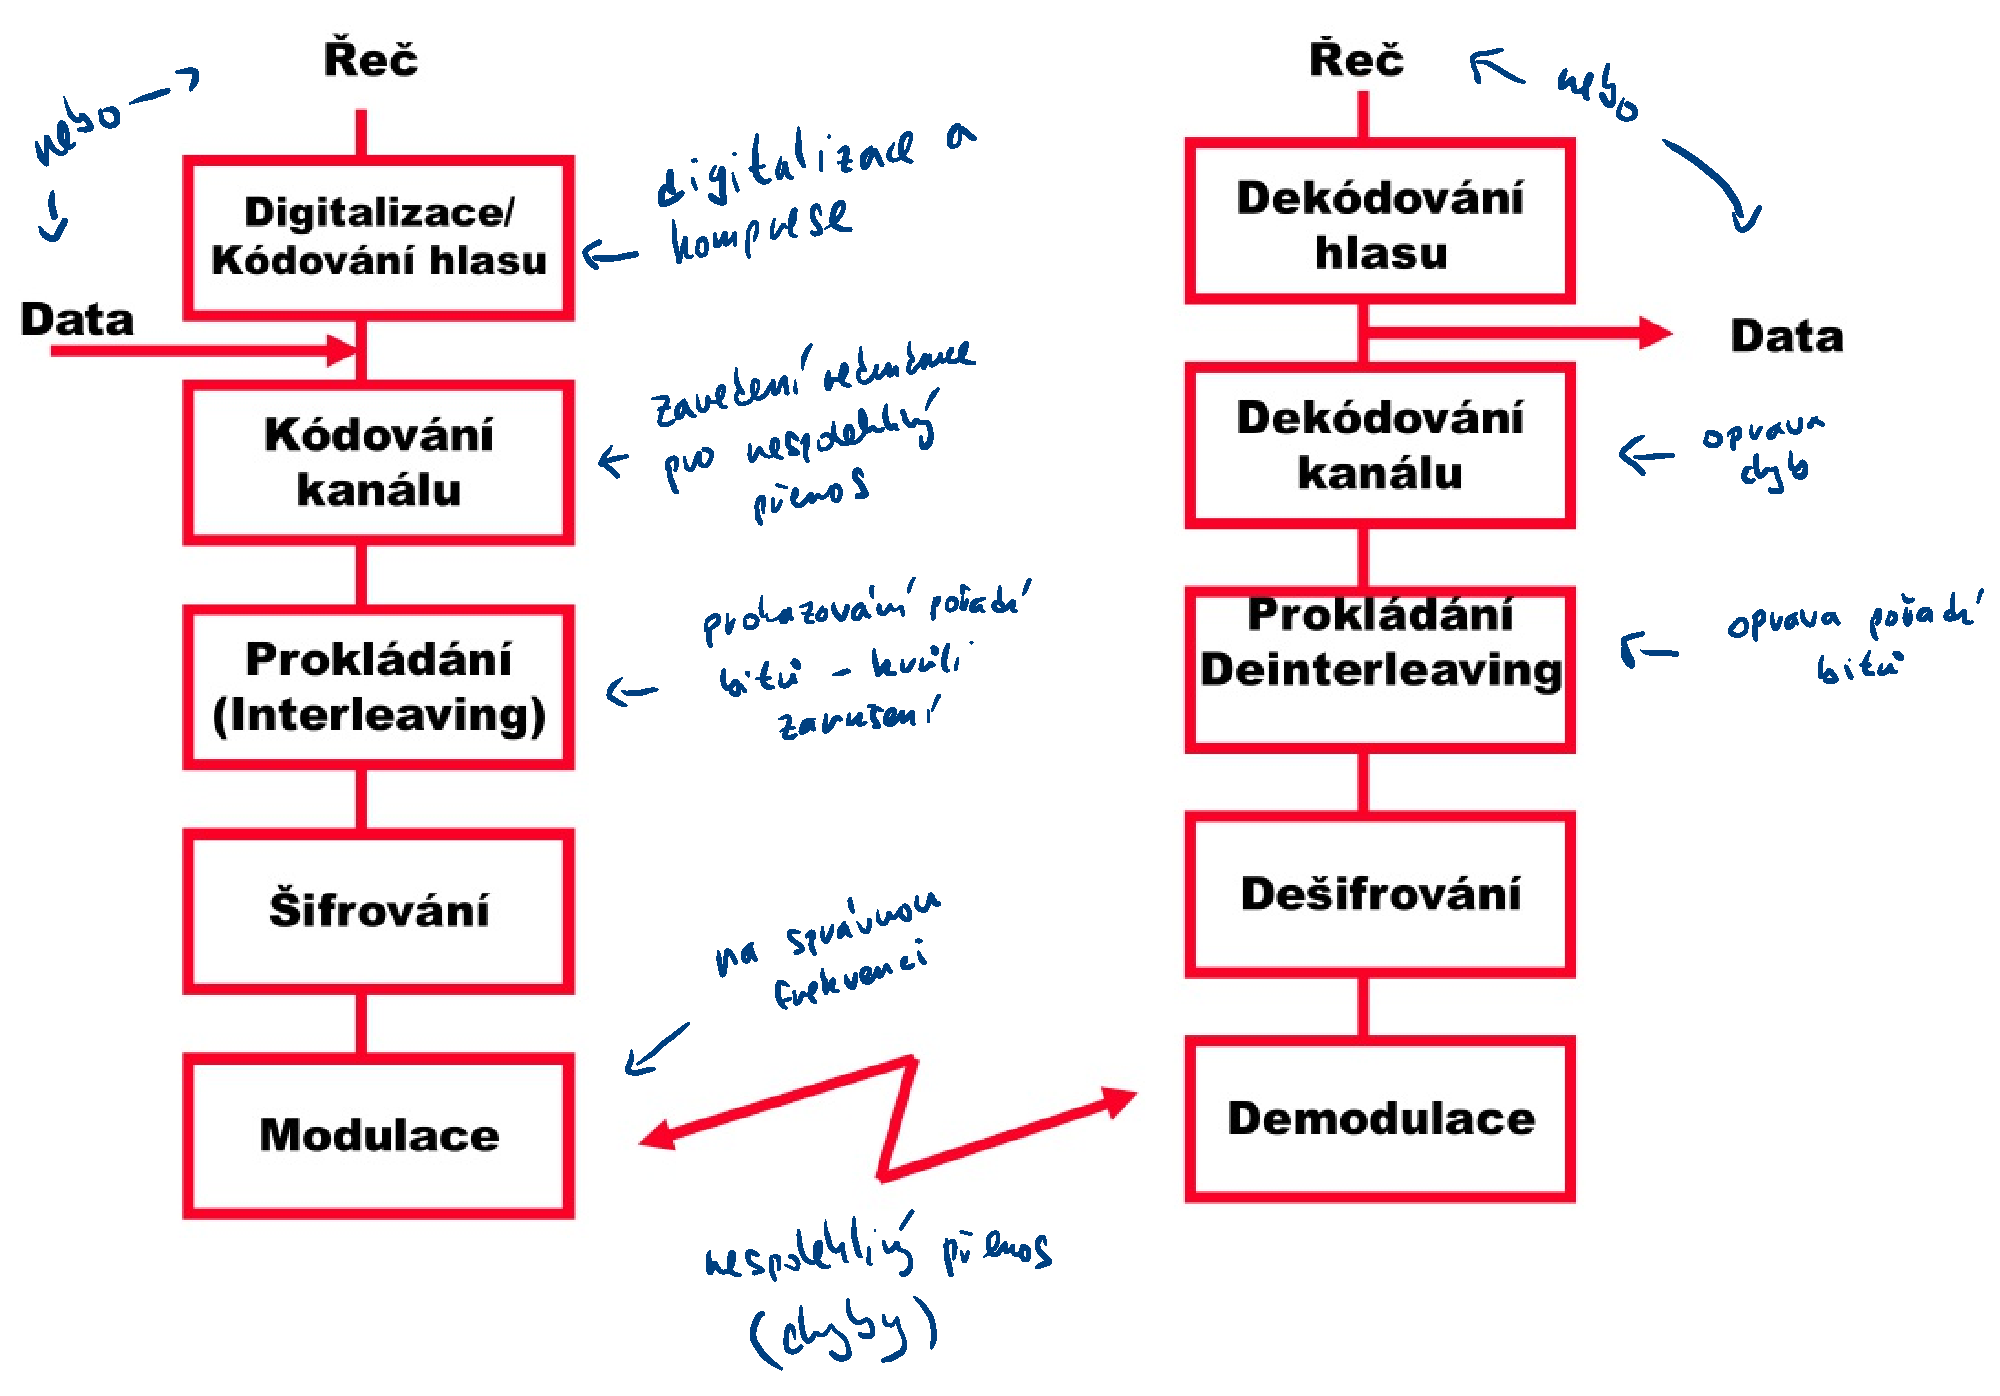
\includegraphics[width=1\linewidth]{bezdratova_komunikace.pdf}
    \caption{Schéma bezdrátové komunikace.}
\end{figure}

%%%%%%%%%%%%%%%%%%%%%%%%%%%%%%%%%%%%%%%%%%%%%%%%%%%%%%%%%%%%%%%%%%%%%%%%%%%%%%%%

\section{Modulace}

\begin{compactitem}
    \item Na straně vysílače: \begin{compactitem}
        \item \textbf{Digitální modulace} (klíčování) -- Vstupní (digitální) signál, je třeba převést na analogový.

        \item \textbf{Analogová modulace} -- Analogový signál je třeba dostat na správnou frekvenci pro přenos (kombinace s nosným signálem).
    \end{compactitem}

    \begin{figure}[H]
        \centering
        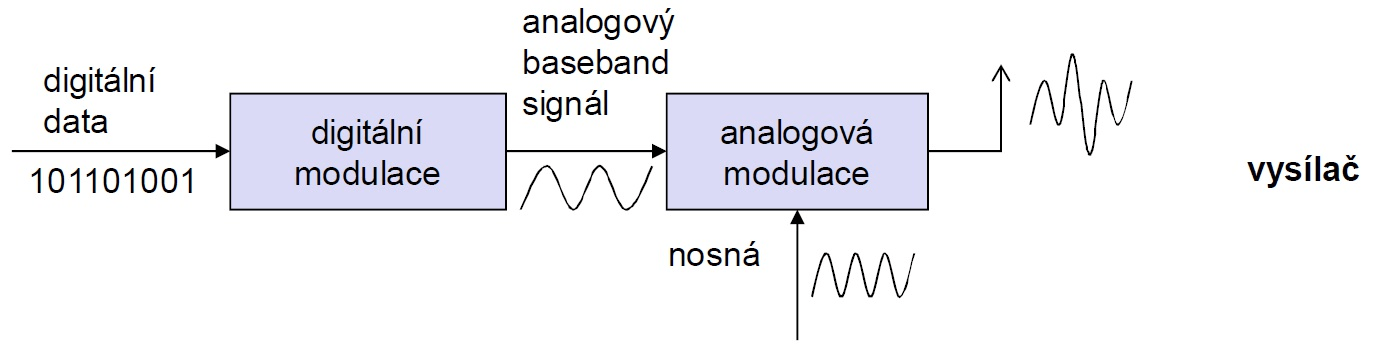
\includegraphics[width=1\linewidth]{modulace.png}
        \caption{Digitální a analogová modulace.}
    \end{figure}

    \item Na straně přijímače: \begin{compactitem}
        \item \textbf{Analogová demodulace} -- Oddělení nosného signálu.

        \item \textbf{Synchronizace a digitalizace} -- Převod analogového signálu na digitální.
    \end{compactitem}

    \begin{figure}[H]
        \centering
        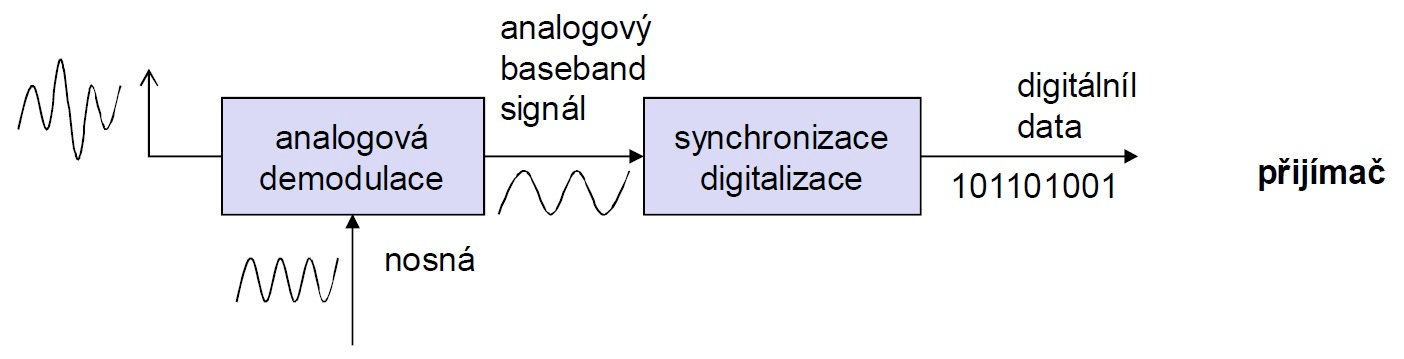
\includegraphics[width=1\linewidth]{demodulace.png}
        \caption{Analogová demodulace a digitalizace.}
    \end{figure}
\end{compactitem}

\subsection{Analogová (de)modulace}

\begin{compactitem}
    \item Vstup: analog, výstup: analog.
    \item Amplitudová modulace (AM, \textit{amplitude modulation}).
    $$ f(x) = C \cdot \sin{(x)} ~,~ C \in \mathbb{R} $$
    \item Frekvenční modulace (FM, \textit{frequency modulation}).
    $$ f(x) = \sin{(C \cdot x)} ~,~ C \in \mathbb{R} $$
    \item Fázová modulace (PM, \textit{phase modulation}).
    $$ f(x) = \sin{(x + C)} ~,~ C \in \mathbb{R} $$
\end{compactitem}

\subsection{Digitální (de)modulace}

\begin{compactitem}
    \item Vstup: digitál, výstup: analog.
    \item Cíl: v jedné sinusovce (signálová jednotka) přenést co nejvíce bitů.
    \item Amplitudová modulace (ASK, \textit{amplitude shift keying}).
    \item Frekvenční modulace (FSK, \textit{frequency shift keying}).
    \item Fázová modulace (PSK, \textit{phase shift keying}). \begin{compactitem}
        \item 2-PSK, 4-PSK, 8-PSK
    \end{compactitem}
    \item Kvadraturní amplitudová modulace (QAM, \textit{quadrature amplitude modulation (shift keying)}). \begin{compactitem}
        \item 8-QAM, 16-QAM, 32-QAM, 64-QAM
    \end{compactitem}
    \item Pro ASK, FSK, 2-PSK: baud rate = bit rate.
\end{compactitem}

%%%%%%%%%%%%%%%%%%%%%%%%%%%%%%%%%%%%%%%%%%%%%%%%%%%%%%%%%%%%%%%%%%%%%%%%%%%%%%%%

\section{Sdílení spektra}

\begin{compactitem}
    \item Jak umožnit více než dvěma koncovým zařízením připojeným ke stejnému přenosovému médiu komunikovat tak, aby se vzájemně nerušili? \begin{compactitem}
        \item Metoda přístupu ke kanálu (\textit{channel access method}).
    \end{compactitem}

    \item Metoda přístupu ke kanálu je založena na sdílení spektra (multiplexing), které umožňuje několika datovým tokům nebo signálům sdílet stejný komunikační kanál nebo přenosové médium. V této souvislosti multiplexování zajišťuje fyzická vrstva.

    \item Mnoho přístupů: \begin{compactenum}
        \item \textbf{Prostorový multiplex} (SDMA, \textit{space-division multiple access}) \begin{compactitem}
            \item Jsme schopni využít 1 frekvenci pro více účastníků, jsou-li fyzicky daleko od sebe.

            \item Je potřeba ochranný interval.
        \end{compactitem}

        \item \textbf{Frekvenční multiplex} (FDMA, \textit{frequency-division multiple access}) \begin{compactitem}
            \item Rozdělení spektra na menší úseky (kanály), které poté přidělujeme účastníkům.
            \item Kanál má 2 atrbitu: šířku a střední frekvenci.
            \item Nevýhoda: plýtvání pásmem, nutnost ochranných intervalů.
        \end{compactitem}

        \item \textbf{Časový multiplex} (TDMA, \textit{time-division multiple access}) \begin{compactitem}
            \item Kanál dostane celé spektrum po určitý čas.
            \item Nelze použít v analogovém vysílání.
            \item Nutná synchronizace.
            \item Jedna nosná, vysoká propustnost.
        \end{compactitem}

        \item \textbf{Časový a frekvenční multiplex} (FTDMA, \textit{frequency and time division multiple access}) \begin{compactitem}
            \item Kombinace časového a frekvenčního multiplexingu.
            \item Každý účastník dostane kanál a časový slot (kde a kdy komunikuje).
            \item Využívá se v GSM.
            \item Nutná časová i frekvenční koordinace.
        \end{compactitem}

        \item \textbf{Kódový multiplex} (CDMA) -- viz dále.

        \item \textbf{Ortogonální multiplex s frekvenčním dělením} (OFDM)-- viz dále.
    \end{compactenum}
\end{compactitem}

\subsection{Kódový multiplex (CDMA)}

\begin{compactitem}
    \item Všichni vysílají na jednom kanálu po celou dobu. \begin{compactitem}
        \item  Nesnažíme se bránit vzájemnému zarušení, to bereme jako součást systému.
    \end{compactitem}

    \item Všichni dostávají signál všech a musí si extrahovat informace pro sebe. \begin{compactitem}
        \item signál všech $\rightarrow$ algoritmus $\rightarrow$ signál účastníka

        \item Každá stanice má své unikátní číslo, pokud přijímač toto číslo zná, může se \uv{naladit} (z čísla derivujeme \uv{náhodný} signál).
    \end{compactitem}

    \item Nevýhoda: \begin{compactitem}
        \item složitost přijímače (potřeba počítač pro kódování / dekódování),
        \item nižší rychlost přenosu.
    \end{compactitem}

    \item Výhoda: \begin{compactitem}
        \item efektivní využití pásma (žádné ochranné intervaly),
        \item žádná koordinace a synchronizace,
        \item odolnost proti rušení a odposlouchávání.
    \end{compactitem}
\end{compactitem}

\begin{figure}[H]
    \centering
    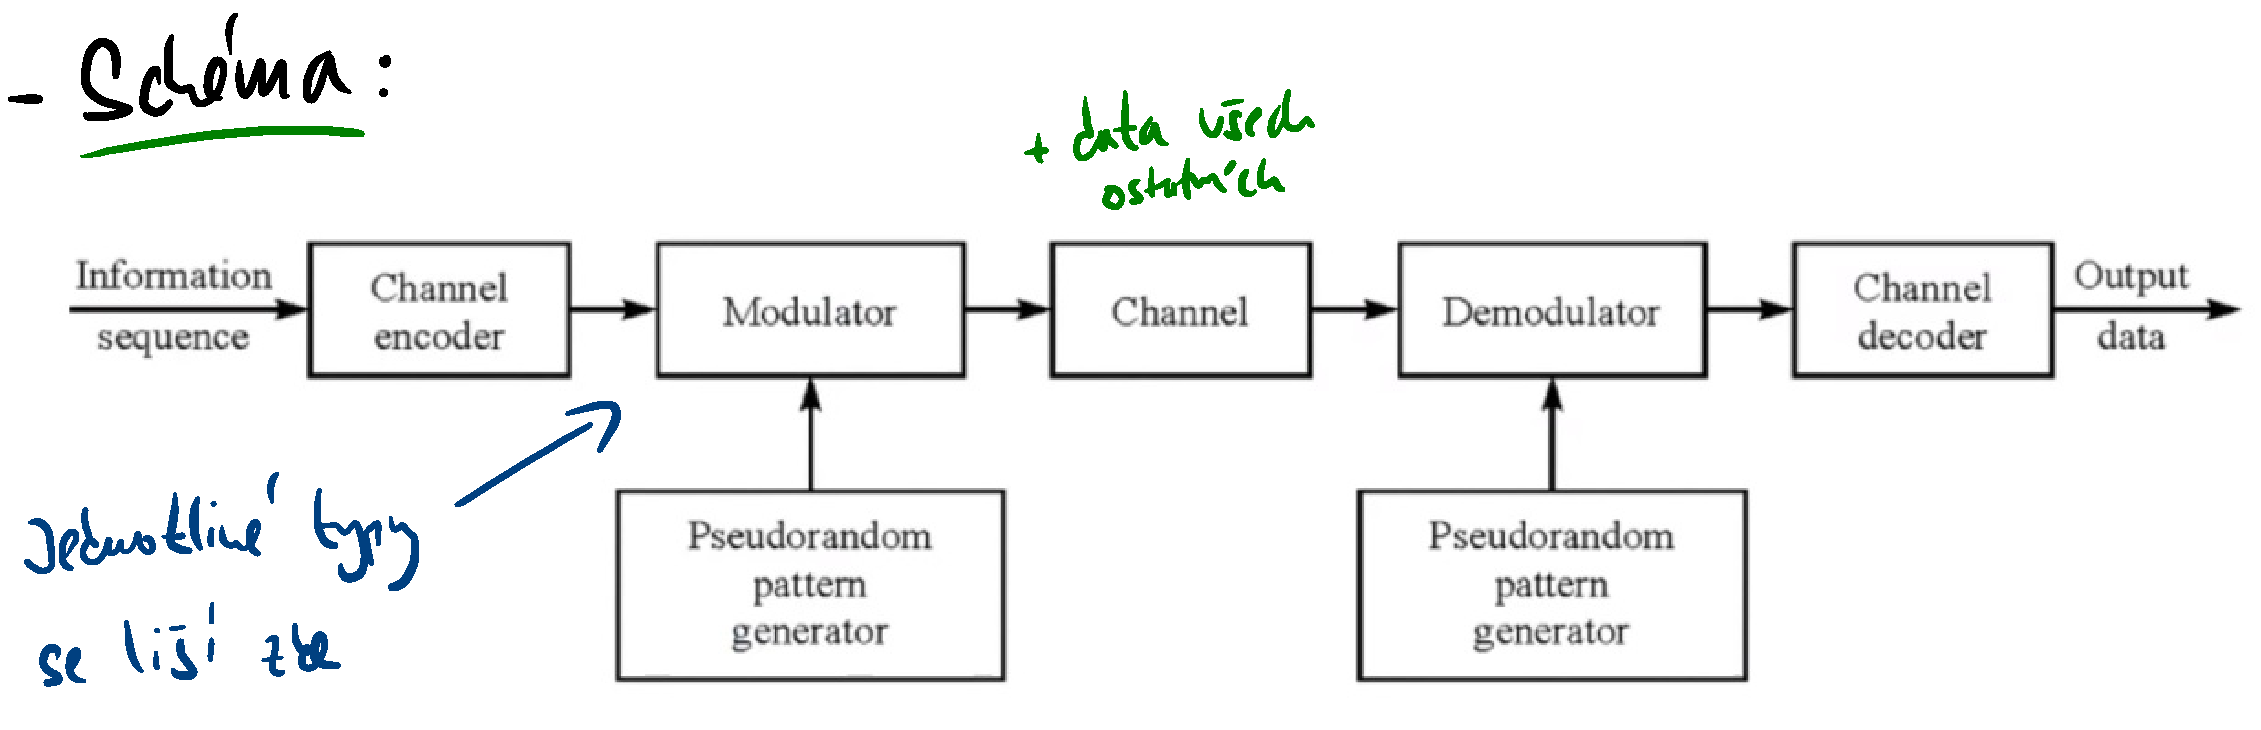
\includegraphics[width=1\linewidth]{cdma.pdf}
    \caption{CDMA schéma.}
\end{figure}

\subsubsection{DSSS (\textit{direct sequence spread spectrum})}

\begin{compactitem}
    \item \uv{Rozprostřené spektrum}.
    \item Užitečný signál $\oplus$ (XOR) vygenerovaný náhodný signál.
    \item Výsledek se namoduluje a posílá.
\end{compactitem}

\begin{figure}[H]
    \centering
    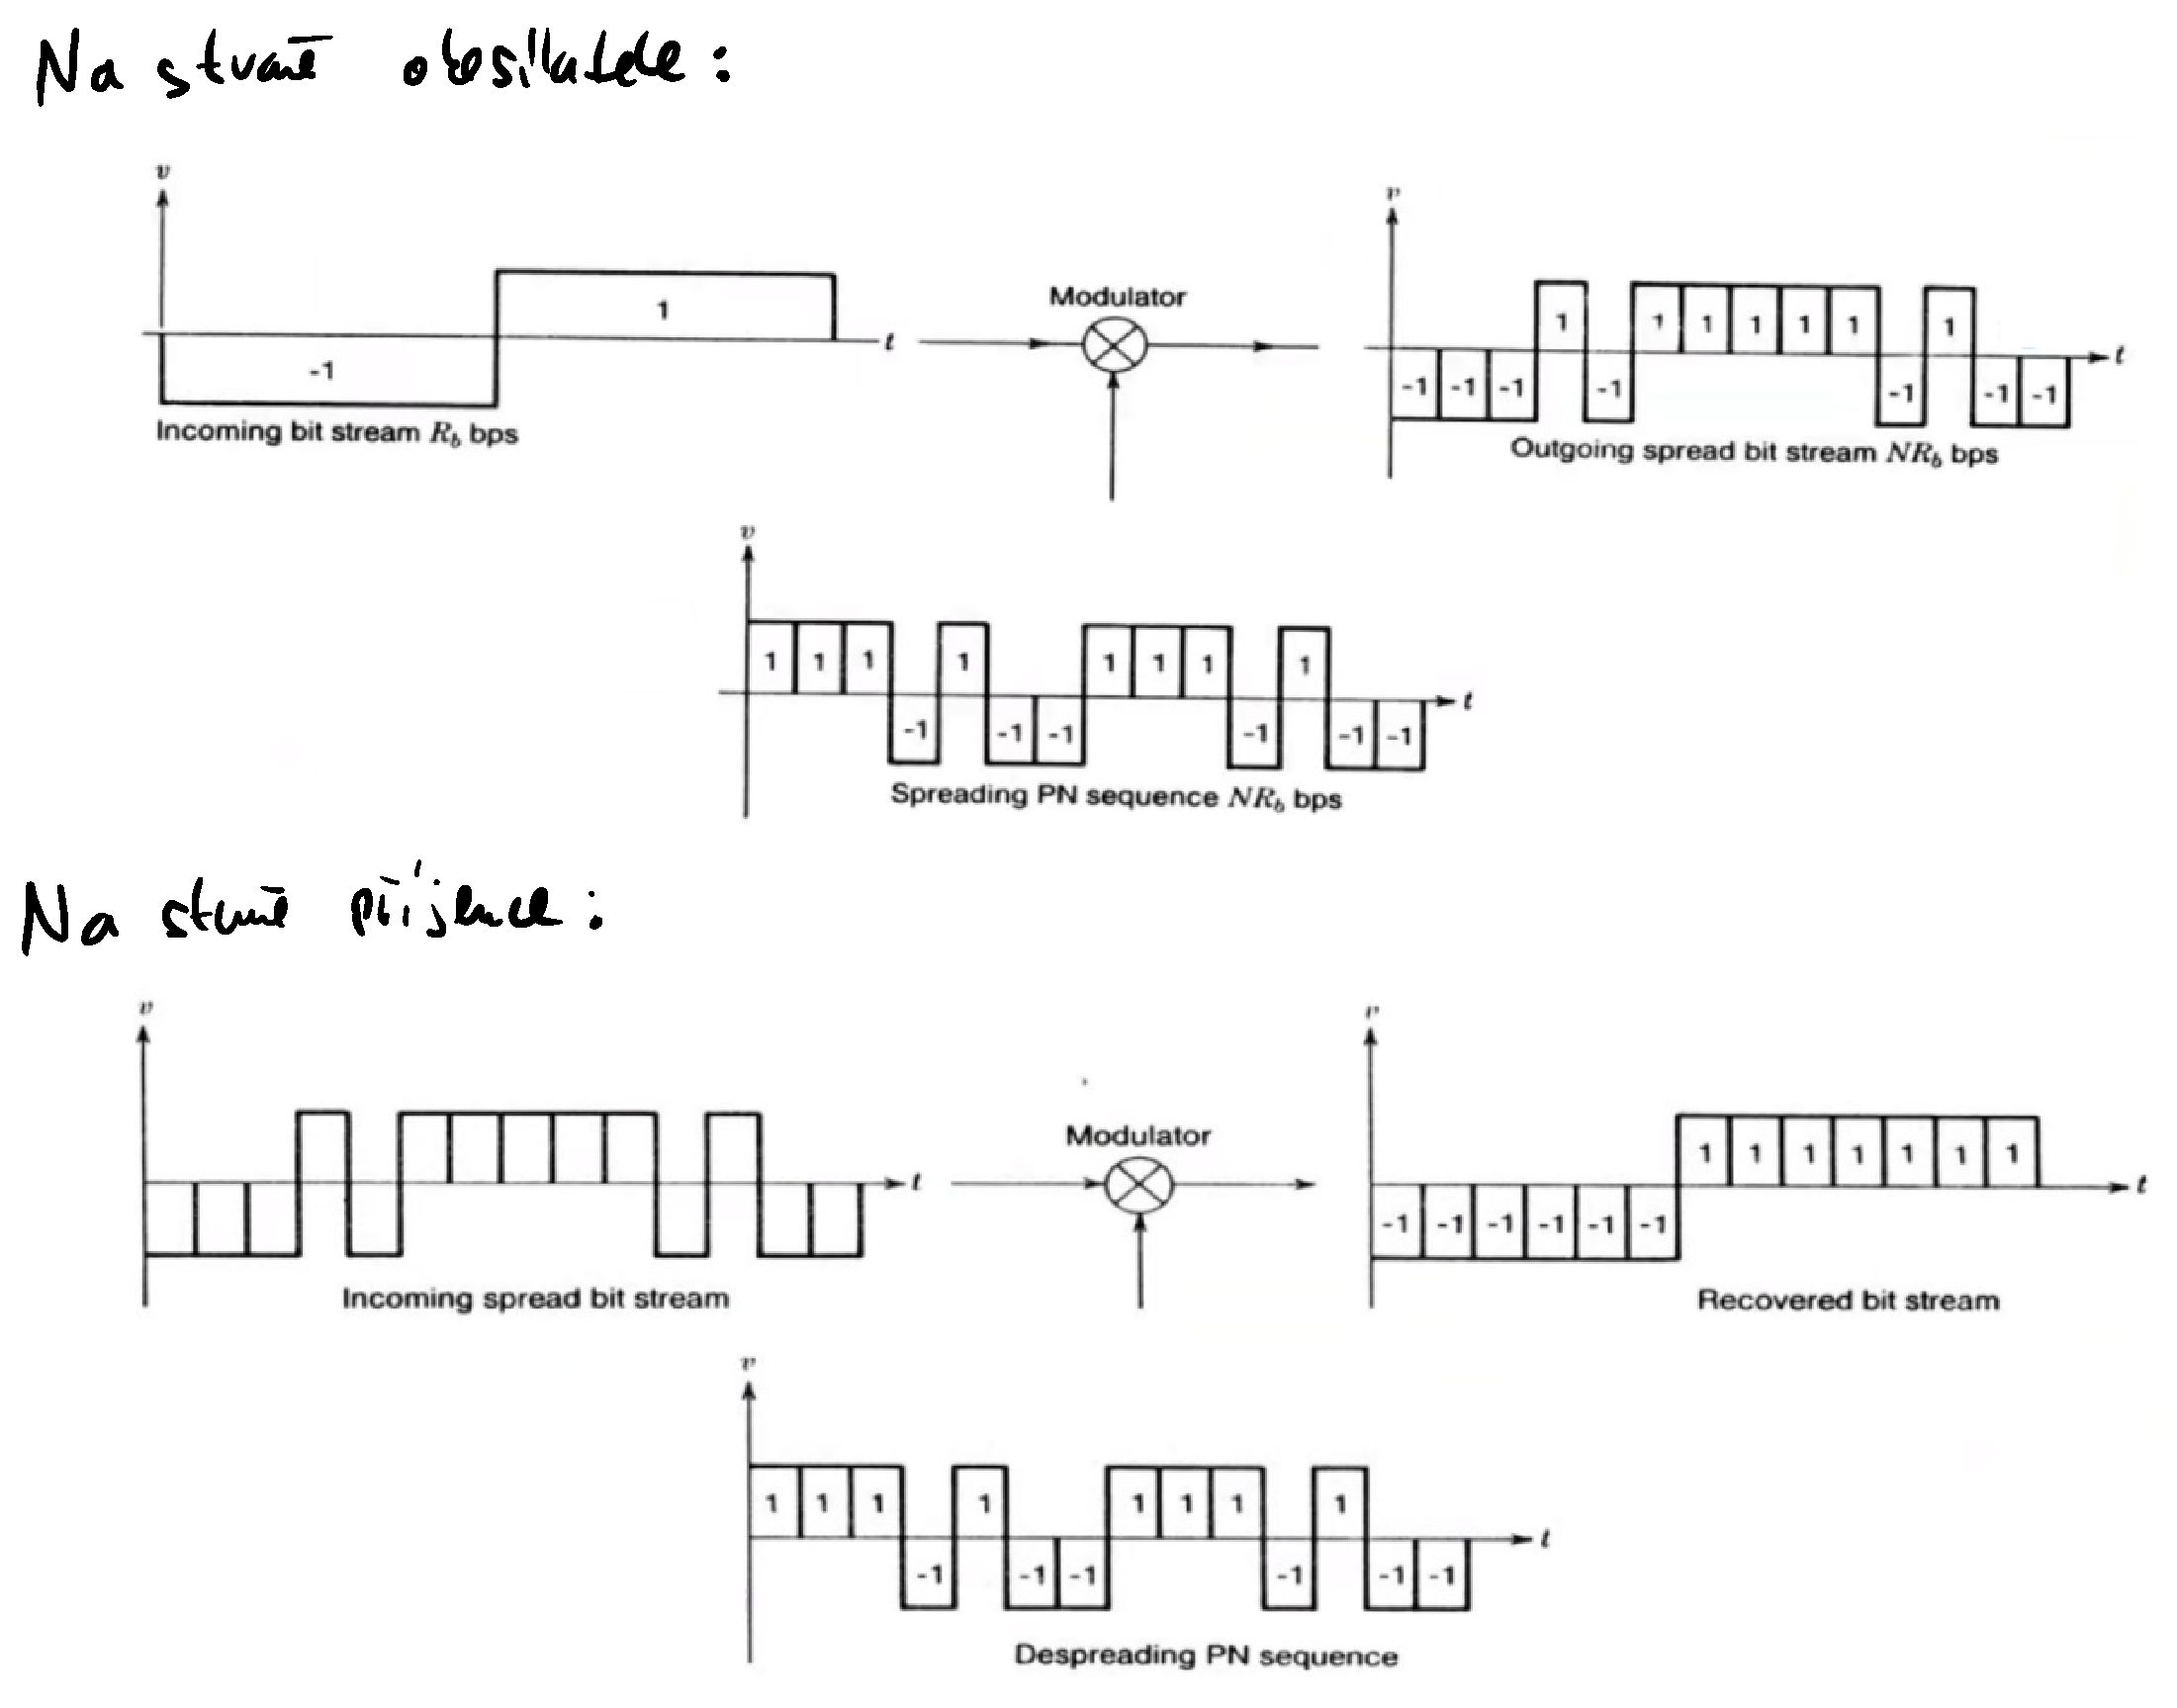
\includegraphics[width=1\linewidth]{dsss.pdf}
    \caption{DSSS.}
\end{figure}

\subsubsection{FHSS (\textit{frequency hopping spread spectrum})}

\begin{compactitem}
    \item Uživatel má k dispozici několik frekvenčních kanálů.
    \item Náhodně vygenerovaná sekvence definuje, kdy se komunikuje přes jaký frekvenční kanál. -- Frekvenční kanály se v průběhu komunikace střídají.
\end{compactitem}

\subsection{Ortogonální multiplex s frekvenčním dělením (OFDM)}

\begin{compactitem}
    \item Ortogonální multiplex s frekvenčním dělením (OFDM, \textit{orthogonal frequency division multiplexing})

    \item Kombinace a FDMA multiplexingu a QAM modulace. \begin{compactitem}
        \item Datový tok celého kanálu se tak dělí na stovky dílčích datových toků jednotlivých subnosných.
        \item Vzniká mnoho úzkých subkanálů, které jsou přenášeny paralelně.
    \end{compactitem}

    \item Subnosné frekvence jsou dále modulovány dle potřeby různě robustními modulacemi (QPSK, 16-QAM, 64-QAM).

    \item Jednotlivé subnosné jsou vzájemně ortogonální, takže maximum každé nosné by se mělo překrývat s minimy ostatních.

    \item Umožňuje, aby se postranní pásma subkanálů překrývala, což šetří pásmo.

    \item Přijímač je schopen oddělit překrývající se subkanály, protože jsou ortogonální.
\end{compactitem}

\begin{figure}[H]
    \centering
    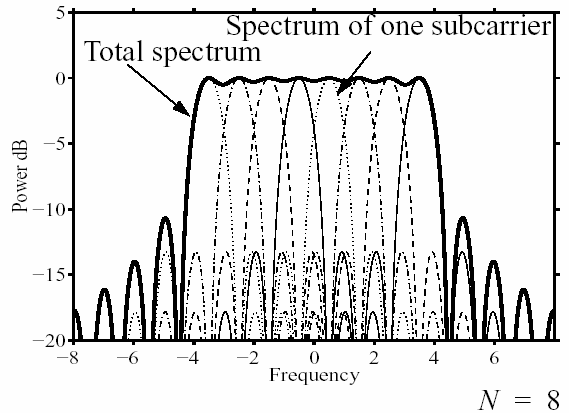
\includegraphics[width=0.6\linewidth]{ofdm.png}
    \caption{Subkanály OFDM, pouze krajní se nemohou překrývat.}
\end{figure}

%%%%%%%%%%%%%%%%%%%%%%%%%%%%%%%%%%%%%%%%%%%%%%%%%%%%%%%%%%%%%%%%%%%%%%%%%%%%%%%%

\section{Bezdrátové lokální sítě}

\begin{compactitem}
    \item \textbf{Výhody} \begin{compactitem}
        \item Velmi flexibilní -- nemusíme natahovat dráty.
        \item Možnost ad-hoc sítí bez předchozího plánování.
        \item Téměř žádné problémy s vedením (historické budovy, požární přepážky).
        \item Robustnější vůči nehodám (nehrozí přerušení vodičů).
    \end{compactitem}

    \item \textbf{Nevýhody} \begin{compactitem}
        \item Nižší přenosová rychlost oproti drátovým sítím (1-10 Mbit/s). \begin{compactitem}
            \item Máme pouze omezené frekvence, na kterých můžeme přenášet data.
        \end{compactitem}
        \item Mnoho proprietárních řešení, standardizace trvá nějakou dobu (např. IEEE 802.11).
        \item Produkty musí dodržovat mnoho různých omezení pro bezdrátové přístroje (frekvenční plánování, výkony, homologace, \dots), vytvořit globální řešení trvá delší dobu.
    \end{compactitem}

    \item \textbf{Cíle návrhu} \begin{compactitem}
        \item Globální provoz. \begin{compactitem}
            \item Historicky problémy vzhledem k různým legislativám ohledně rádiového vysílání v jednotlivých státech.
        \end{compactitem}
        \item Nízká spotřeba pro provoz z baterií.
        \item Bezpečnost -- Bezdrátové sítě se snáze odposlouchávají, než drátové, proto je šifrování nutnost.
        \item Transparentnost k vyšším protokolům. \begin{compactitem}
            \item Např. TCP/IP neví jestli běží po drátové/bezdrátové technologii.
        \end{compactitem}
    \end{compactitem}

    \item Jako fyzické médium se používá \textbf{rádiový přenos} (typicky bezlicenční pásmo 2,4\,GHz), ačkoliv historicky byl ve hře i infračervený přenos.

    \item \textbf{Adhoc sítě} \begin{compactitem}
        \item Decentralizovaný typ bezdrátové sítě, kde nezávisí na předem existující infrastruktuře, jako jsou směrovače v kabelových sítích nebo \textit{access pointy} v bezdrátových sítích.
        \item Jako ad hoc síť se typicky označuje množina sítí, kde jsou všechna zařízení rovnocenná a volně spojitelná s jakoukoliv jinou ad hoc sítí v dosahu.
        \item Určité uzly podílí na předávání dat jiným uzlům a jejich určení je prováděno dynamicky na základě síťové konektivity.
    \end{compactitem}

    \item \textbf{Infrastrukturní síť} \begin{compactitem}
        \item Máme předem danou infrastrukturu (směrovače, \textit{access pointy}), ke které se připojují klienti.
    \end{compactitem}
\end{compactitem}

%%%%%%%%%%%%%%%%%%%%%%%%%%%%%%%%%%%%%%%%%%%%%%%%%%%%%%%%%%%%%%%%%%%%%%%%%%%%%%%%

\section{WiFi}

\begin{compactitem}
    \item WiFi (\textit{wireless local area network}), několik verzí standardu IEEE 802.11.

    \item Specifikuje fyzickou vrstvu ($L_0$) a vrstvu síťového rozhraní ($L_1$) v TCP/IP stacku, resp. ISO/OSI.

    \item Fyzická vrstva -- fyzické médium (rádiové, infračervené vysílání) + vrstva konvergence, která zapouzdřuje médium.

    \item Vrstva síťového rozhraní -- přístup k fyzickému médiu, fragmentace, šifrování, detekce a korekce chyb.
\end{compactitem}

\begin{figure}[H]
    \centering
    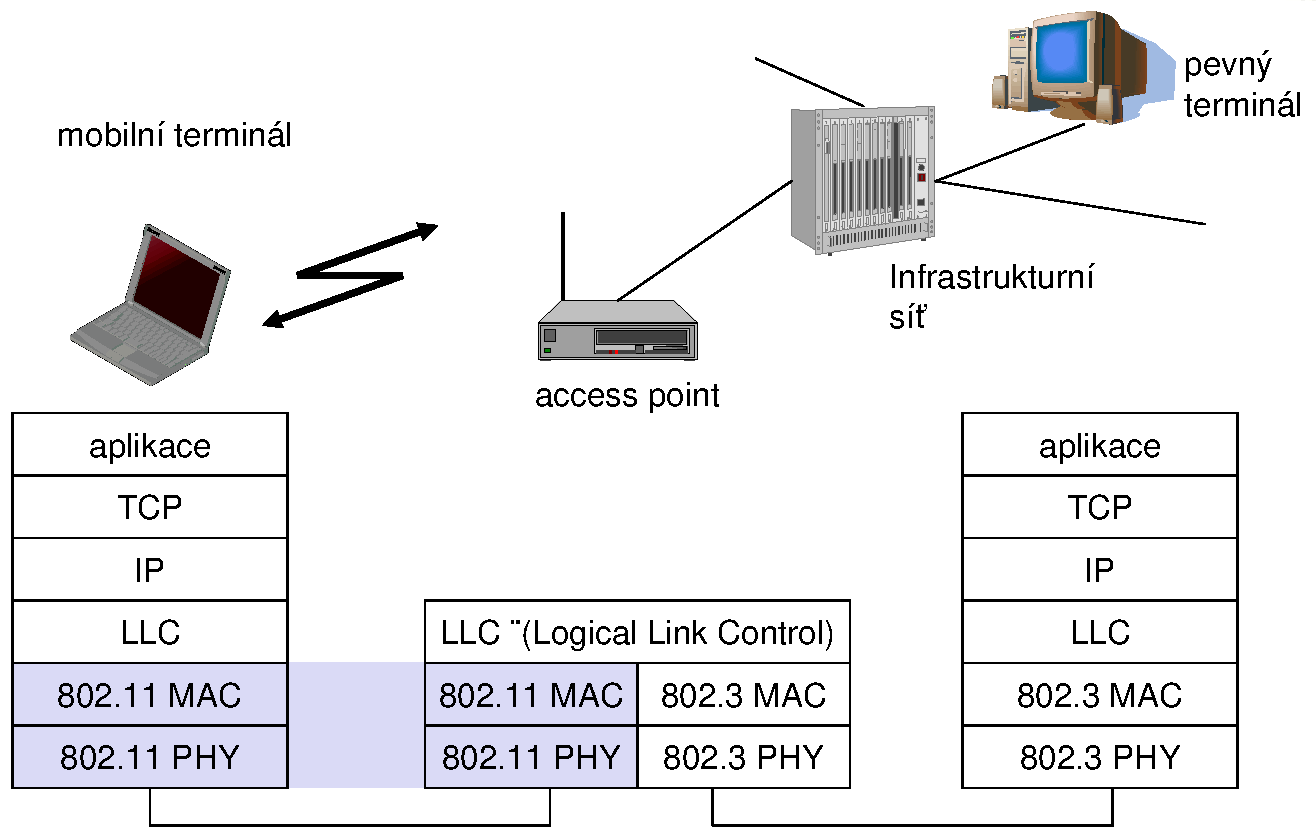
\includegraphics[width=0.75\linewidth]{wifi-architektura.pdf}
    \caption{IEEE 802.11 WiFi architektura, PHY značí fyzickou vrstvu, MAC síťového rozhraní.}
\end{figure}

\subsection{IEEE 802.11}

\begin{compactitem}
    \item Pásmo: 2,4\,GHz.

    \item Maximální rychlost: 2\,Mbitps.

    \item Fyzická vrstva: \begin{compactitem}
        \item rádiové kanály, multimplexing CDMA (\textit{code division multiple access}), konkrétně DSSS (\textit{direct sequence spread spectrum}) -- přežilo,
        \item rádiové kanály, CDMA, konkrétně FHSS -- zahynulo.
        \item infračervené kanály -- zahynulo.
    \end{compactitem}

    \item Fyzická vrstva, která přežila, má 11 kanálů o šířce 22 MHz, které se překrývají (netypické).
\end{compactitem}

\subsection{IEEE 802.11a}

\begin{compactitem}
    \item Americký nástupce (použití pouze USA) 802.11.

    \item Frekvenční pásmo: 5,0\,GHz.
    \item Maximální rychlost: 54\,Mbitps
    \item Maximální dosah: 100\,m mimo budovy, 10\,m v budově.

    \item Cíl: \begin{compactitem}
        \item přidělení nového frekvenčního pásma, které není tak vytížené (není zpětná kompatibilita),
        \item dosáhnutí vyšší rychlosti,
        \item odstranění infračervených a rádiových FHSS kanálů.
    \end{compactitem}

    \item Jak dosahuje zrychlení? \begin{compactitem}
        \item Díky tomu, že není zpětně kompatibilní, může používat nové sdílení spektra OFDM.
    \end{compactitem}

    \item Modulace: 2-PSK, 4-PSK, 16-QAM, 64-QAM.

    \item Zhodnocení: \begin{compactitem}
        \item není zpětně kompatibilní,
        \item je rychlé,
        \item má menší dosah (kvůli vyšší frekvenci, která má vyšší útlum).
    \end{compactitem}
\end{compactitem}

\subsection{IEEE 802.11b}

\begin{compactitem}
    \item Evropský nástupce (použití celosvětově) 802.11.

    \item Frekvenční pásmo: 2,4\,GHz.
    \item Maximální rychlost: 11\,Mbitps.
    \item Maximální dosah: 300\,m mimo budovy, 30\,m v budově.

    \item Cíl: \begin{compactitem}
        \item původní frekvenční pásmo,
        \item dosáhnutí vyšší rychlosti,
        \item odstranění infračervené a rádiové FHSS fyzické vrstvy,
        \item zpětná kompatibilita (ale pouze 1 fyzická vrstva).
    \end{compactitem}

    \item Sdílení spektra DSSS (rozprostírací sekvence je tzv. Barkerův kód).

    \item Jak dosahuje zrychlení? \begin{compactitem}
        \item Původní modulační schémata DBPSK, DQPSK pro rychlost 2\,Mbitps.
        \item Nové modulační schéma CCK pro 11\,Mbitps.
    \end{compactitem}

    \item Zhodnocení: \begin{compactitem}
        \item je zpětně kompatibilní,
        \item není tak rychlé jako 802.11a,
        \item ale má větší dosah než 802.11a.
    \end{compactitem}
\end{compactitem}

\subsection{IEEE 802.11g}

\begin{compactitem}
    \item Frekvenční pásmo: 2,4\,GHz.
    \item Maximální rychlost: 54\,Mbitps
    \item Rychlé a má velký dosah.

    \item Cíl: \begin{compactitem}
        \item všechno dobré z 802.11a importovat do 802.11b, tj. zachovat frekvenci 2,4\,GHz,
        \item sdílení spektra OFDM,
        \item zpětná kompatibilita s 802.11b.
    \end{compactitem}
\end{compactitem}

\begin{figure}[H]
    \centering
    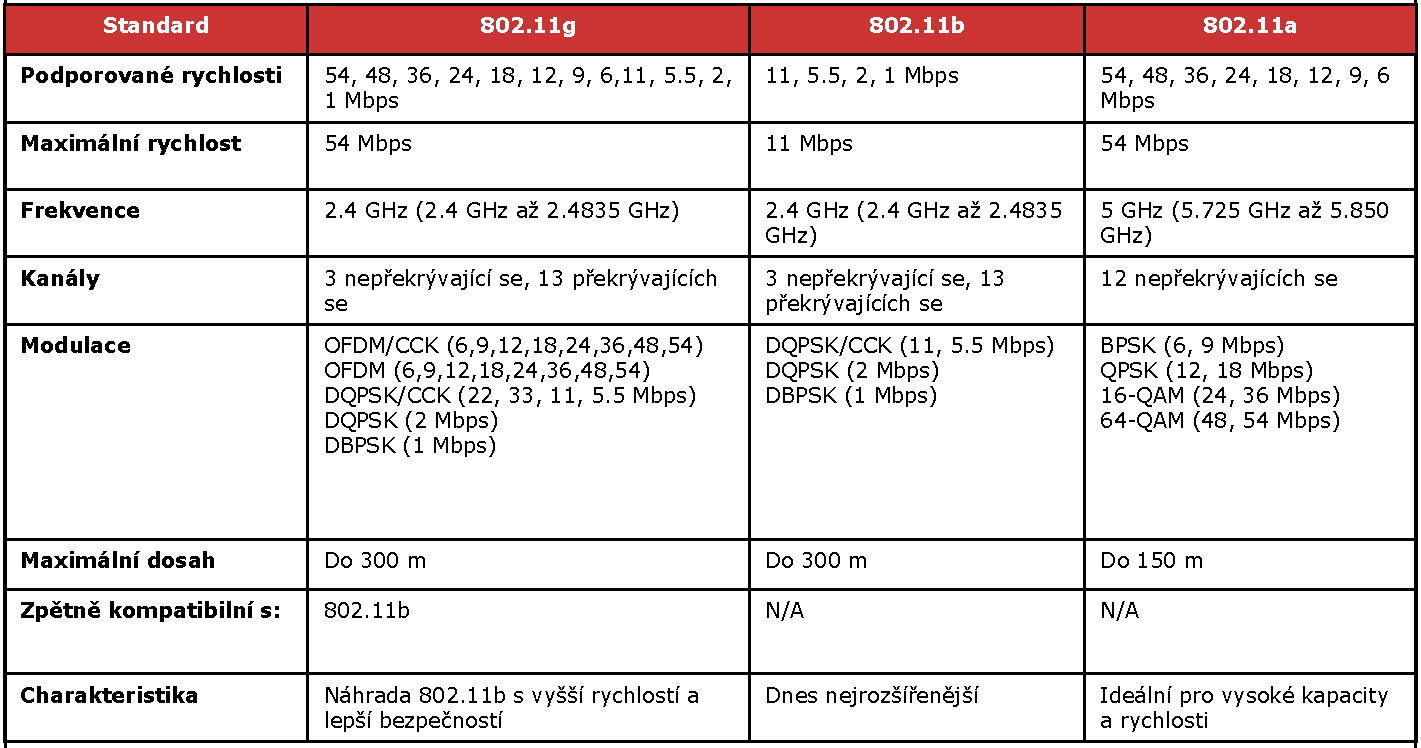
\includegraphics[width=1\linewidth]{802_11_abg.pdf}
    \caption{Srovnání standardů IEEE 802.11 a, b a g.}
\end{figure}

%%%%%%%%%%%%%%%%%%%%%%%%%%%%%%%%%%%%%%%%%%%%%%%%%%%%%%%%%%%%%%%%%%%%%%%%%%%%%%%%

\section{Bluetooth}

\begin{compactitem}
    \item Bluetooth, \textit{wireless personal area network}.

    \item Typický případ použití: komunikace mezi různými zařízeními stejného uživatele. \begin{compactitem}
        \item Propojení počítačů, periferie, mobilní telefon (náhrada kabelů).
    \end{compactitem}

    \item Univerzální rádiový prostředek pro bezdrátové propojení v ad-hoc sítích.

    \item Krátký dosah (10 m) a nízká spotřeba (bezlicenční pásmo 2,4\,GHz).

    \item Požadavky: přenos hlasu a dat (datová rychlost cca. 1\,Mbitps).

    \item Vlastnosti: \begin{compactitem}
        \item Frekvenční pásmo: 2,4\,GHz (79 rádiových kanálů, vzdálenost 1\,MHz).
        \item Modulace: G-FSK (\textit{gaussian frequency-shift keying}).
        \item Multiplexing: FHSS (\textit{frequency hopping spread spectrum}).
        \item Datové přenosy -- asynchronní, bez navázání spojení.
        \item Hlasové přenosy -- synchronní, navazování spojení, forward error correction, vadné pakety se neposílají znovu.
    \end{compactitem}

    \item Topologie: hvězdicová, \uv{pikonet} / \uv{scatternet}.

    \item Zabezpečení: \begin{compactitem}
        \item PIN $\rightarrow$ šifrovací klíč (128 bit) $\rightarrow$ šifrovaná komunikace.
    \end{compactitem}

    \item Historicky problémy s kompatibilitou a párováním.
\end{compactitem}

\subsection{Pikonet}

\begin{compactitem}
    \item Sbírka zařízení, které se nacházejí ve vzájemné blízkosti podle
    principu ad-hoc.

    \item Jedno z nich pracuje jako master a ostatní jako slave po celou dobu života pikonetu.

    \item Master určuje hopping sekvenci, slave se musí zasynchronizovat.

    \item Každý pikonet má svou hopping sekvenci.

    \item Uzel se stane účastníkem pikonetu tím, že se zasychnchronizuje na hopping sekvenci.

    \item Každý pikonet má jeden master uzel a v jednom okamžiku až 7 aktivních slave uzlů (ale více než 200 může být ve stavu \uv{zaparkovaný}).

    \item Všechna zařízení v pikonetu mají stejnou hopping sekvenci.
\end{compactitem}

\begin{figure}[H]
    \centering
    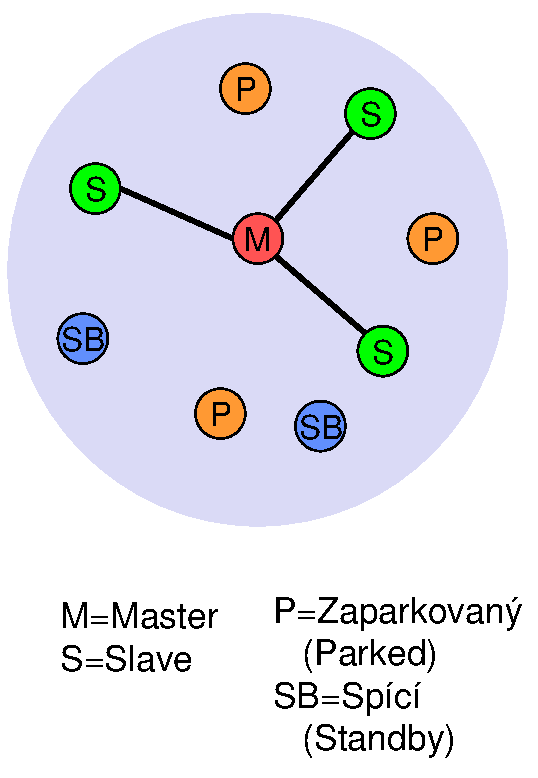
\includegraphics[width=0.4\linewidth]{pikonet.pdf}
    \caption{Příklad pikonetu.}
\end{figure}

\subsection{Scatternet}

\begin{compactitem}
    \item Propojení několika blízkých pikonetů prostřednictvím sdílení uzlů master nebo slave. \begin{compactitem}
        \item Uzel může být slave v jednom pikonetu a master ve druhém.
    \end{compactitem}

    \item Komunikace mezi pikonety. \begin{compactitem}
        \item Uzel přeskakuje tam a zpátky mezi pikonety.
    \end{compactitem}

    \item Ne každý uzel se dokáže připojit do více pikonetů, většinou pouze laptop nebo smartphone.
\end{compactitem}

\begin{figure}[H]
    \centering
    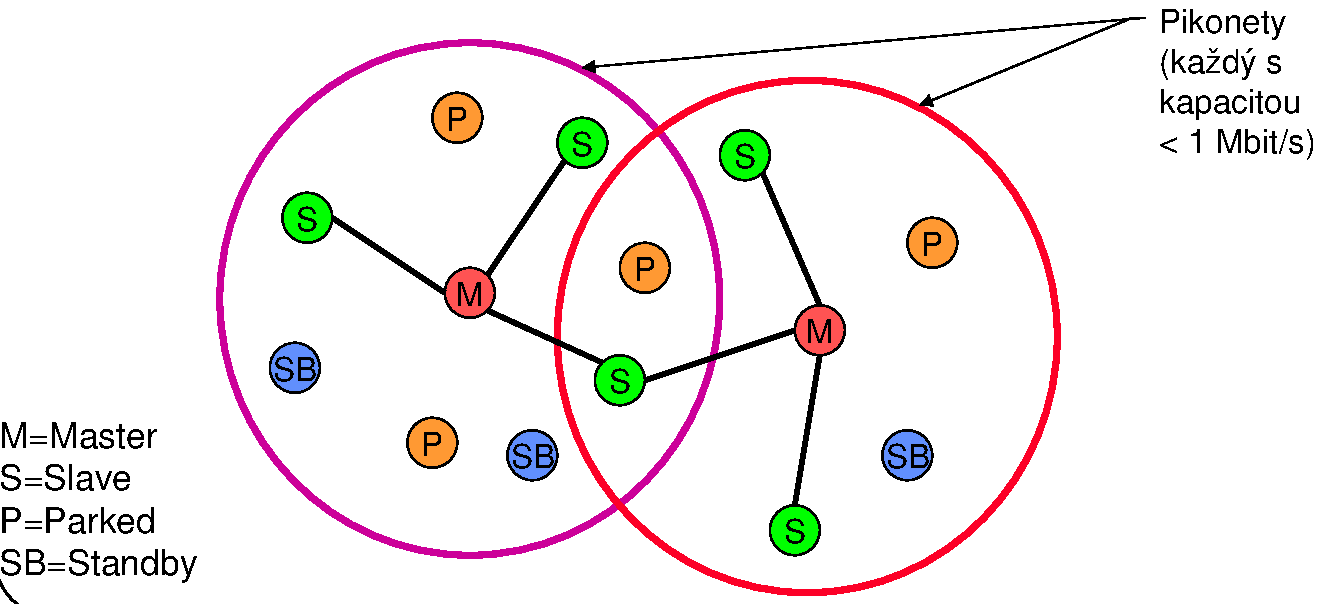
\includegraphics[width=0.9\linewidth]{scatternet.pdf}
    \caption{Příklad scatternetu.}
\end{figure}

\subsection{Protokol stack}

\begin{compactitem}
    \item Service discovery protokol -- Protokol pro zjištění nabízených služeb, hledá uzly v rádiovém dosahu.
\end{compactitem}

\begin{figure}[H]
    \centering
    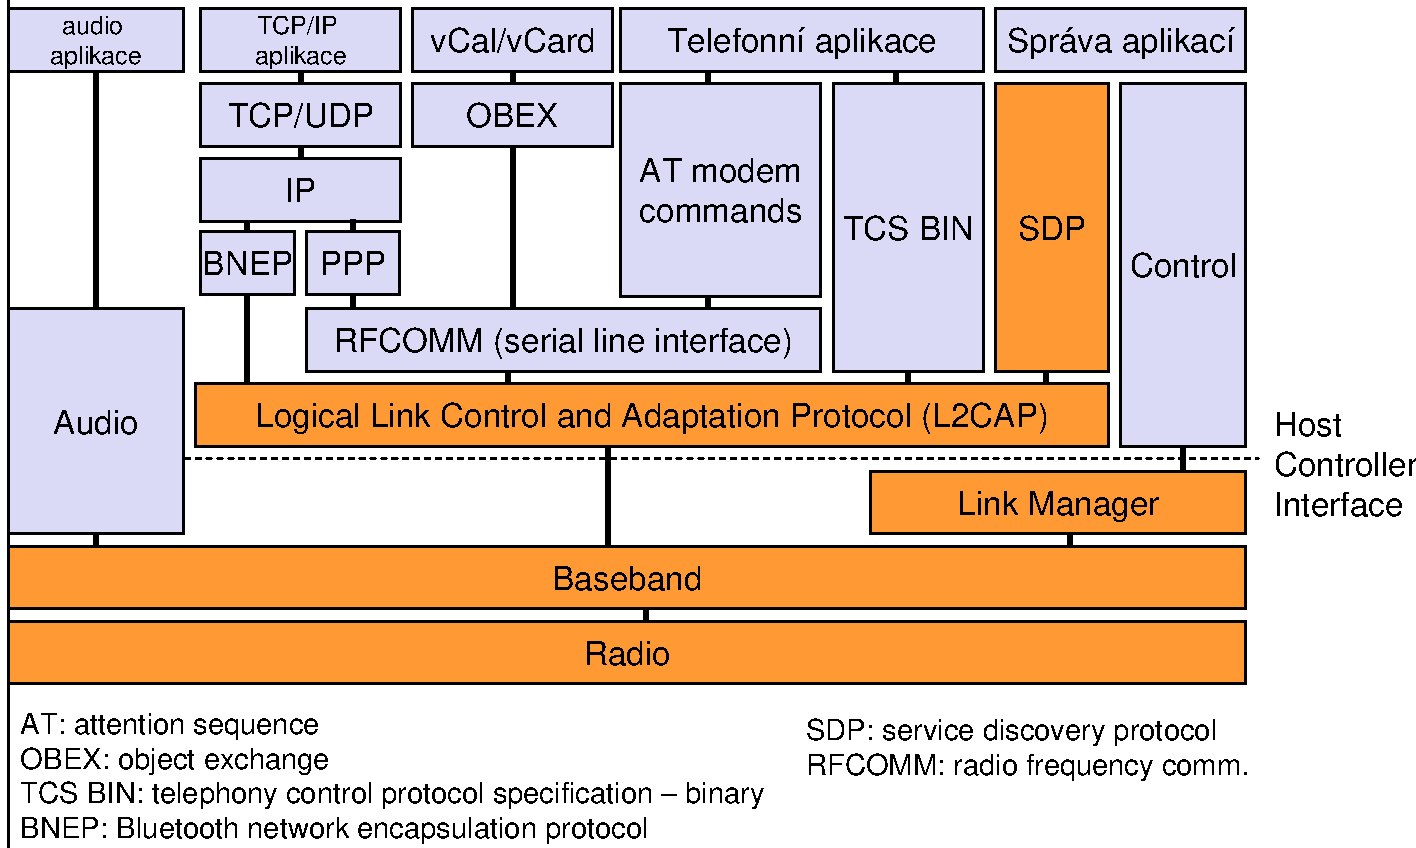
\includegraphics[width=1\linewidth]{bluetooth_protocol_stack.pdf}
    \caption{Bluetooth protokol stack.}
\end{figure}
